
\chapter{Motivação}
Neste cápitulo será abordada a motivação por trás da pesquisa produzida. Na primeira seção, será falado um pouco sobre a grande adoção das práticas ágeis pela indústria. Já na segunda seção, será abordada a falta de estudos voltados para o contexto Recifense. A terceira discorre sobre o artigo base que serviu de motivação para este trabalho. A última seção contém as perguntas de pesquisa que este trabalho tenta responder.

\section{A grande adoção de CI e CD}
As práticas de integração e \emph{deployment} contínuos (\emph{Continuous Integration} e \emph{Continuous Deployment}) já são muito difundidas e utilizadas por empresas de tecnologia em todo o mundo. Segundo \cite{stateAgileReport2020}, 95\% dos participantes reportaram que sua organização pratica metodologias ágeis de desenvolvimento e 55\% utilizam a técnica de integração continua. Também nesta mesma pesquisa foi encontrado que 36\% utilizam a técnica de \emph{deployment} contínuos. 

Estes números elevados são causados principalmente pelos benefícios que a utilização destas técnicas trazem para a equipe e para o produto em desenvolvimento. Ainda de acordo com \cite{stateAgileReport2020}, entre as razões para adoção de CI/CD, as principais são aceleração de entregas de software (71\%), e aumentar a produtividade (51\%) e a qualidade do software (42\%). 

Especificamente sobre integração contínua, a prática hoje em dia já é bastante estudada difundida na indústria. O estudo \cite{hilton2016} comenta que desenvolvedores envolvidos se sentem mais produtivos quando utilizam a prática e dão mais valor aos testes automáticos.  Já com relação a \emph{deployment} contínuo, o estudo \cite{savor2015} mostra que seu uso traz maior qualidade ao software que está sendo produzido. 

\section{A falta de estudos no contexto Recifense}

Ainda há, no entanto, uma grande falta de estudos a respeito de como essas práticas se exportaram para as grandes empresas \cite{empiricalStudy2016}, inclusive em Recife, um dos grandes polos tecnológicos do Brasil. Somente no Porto Digital, localizado na capital pernambucana, há cerca de 330 empresas e 11 mil trabalhadores com faturamento anual de R\$ 2,3 bilhões somente em 2019 \cite{portoDigital}.

% TODO adicionar artigos sobre recife(?)

\section{O artigo base}
Com o objetivo de entender um pouco mais sobre o estado das práticas de CI/CD no contexto de Recife, nos baseamos no estudo \cite{empiricalStudy2016}, que busca entender como as práticas geralmente associadas a \emph{Continuous Deployment} acharam o seu caminho na indústria européia e norte-americana. Para tal, foi utilizado um método misto de estudo empírico baseado em um pré-estudo na literatura, entrevistas qualitativas com 20 participantes e uma entrevista quantitativa que recebeu 187 respostas. A ideia era questionar até que ponto a sabedoria na area estava dominada por peculiaridades de um pequeno grupo de grandes empresas, como Facebook e Google.

Durante o trabalho os autores definem a \emph{stairway to heaven} (escada para o céu, em tradução livre), que tem como objetivo definir um caminho de evolução das empresas para um estágio de entregas sofisticado. Esta permeia práticas de integração contínua, \emph{deployment} contínuo e entregas parciais e 

\begin{figure}[ht]
\begin{center}
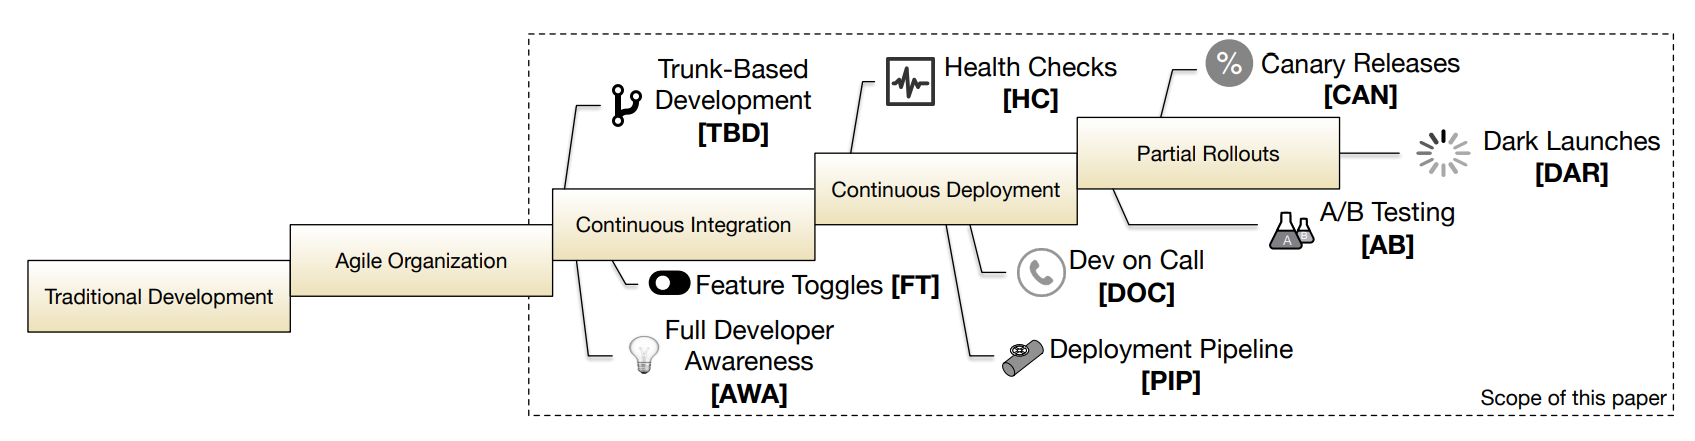
\includegraphics[width=\textwidth]{stairway_to_heaven.png}
\end{center}
\caption[Stairway to Heaven]{
    A escada de evolução denominada "Stairway to Heaven" proposta pelo artigo base.
    Fonte: Schermman et al (2016)
}\label{fig_exe}

\end{figure}

Com este caminho definido, os autores do artigo montaram as entrevistas qualitativas e quantitativas baseadas nas práticas que surgiram em cada degrau da evolução. O interessante da abordagem dos autores foi o roteiro consistir de perguntas sobre o processo utilizado, sem perguntar diretamente se o entrevistado utiliza determinada prática. Isso faz com que os resultados baseiem-se em um conjunto contido de definições, excluindo concepções diversas que pessoas diferentes possam ter a respeito de um mesmo assunto.

\section{Perguntas de pesquisa} 
Assim, a grande adoção da indústria mundial das práticas de CI/CD, aliado a pequena quantidade de trabalhos a respeito no contexto recifense e a excelente metodologia proposta pelo artigo de Schermman et al \cite{empiricalStudy2016} foram as principais motivações para o desenvolvimento deste trabalho. Para este as seguintes perguntas de pesquisa foram formadas:

\begin{enumerate}
\item Quais as práticas de CI/CD são utilizadas pelas empresas em Recife?
\item O cenário de CI/CD nas empresas em recife segue o \emph{stairway to heaven} proposto no artigo?
\item Quais são os princípios e práticas subjacentes que governam a adoção de CD na indústria?
\end{enumerate}

Para responder as perguntas acima foi decido reaplicar a pesquisa qualitativa do artigo \cite{empiricalStudy2016} com desenvolvedores recifenses, baseando-se também na mesma lista de definições de cada uma das práticas envolvidas no "stairway to heaven". A pesquisa qualitativa neste contexto foi considerada fundamental para garantir que os entrevistados entendessem claramente as perguntas e excluir possíveis entendimentos errados de termos em inglês, linguagem não nativa de todos os participantes. Vale salientar que não foi replicado a pesquisa quantitativa presente no artigo base, mas esta pode servir como um trabalho futuro a este.

Além disso, as perguntas 1 e 3 são bem parecidas com as perguntas de pesquisa do artigo base, mas incluindo a técnica de \emph{Continuous Integration}. Não obstante, uma terceira pergunta foi adicionada (\emph{RQ2}), que foca na escada de evolução proposta pelo artigo. Ela tenta responder se a \emph{stairway to heaven} é seguida no contexto de Recife, visto que, no outro, os próprios autores já refutaram esta definição com os seus resultados.


